\documentclass[a4paper,11pt]{article}


\usepackage[utf8]{inputenc}     
\usepackage[T1]{fontenc}        
\usepackage[ngerman]{babel}  
\usepackage{fontspec}   
\usepackage{geometry}   
\usepackage{titlesec}  
\usepackage{setspace}
\usepackage{fancyhdr} 
\usepackage{lipsum}
\usepackage{wrapfig}
\usepackage{ragged2e}
%\usepackage{hyperref}


\fancyhf{}
\fancyfoot[C]{\thepage}
\thispagestyle{empty}
\fancyhead[L]{Gruppe 04}
\fancyhead[C]{\Versuchnummer {} \Versuch}
\fancyhead[R]{\Abgabedatum}

\geometry{left=3cm, right=3cm, top=3cm, bottom=3cm}

\usepackage{xcolor}             
\usepackage{graphicx}           


\usepackage{ragged2e}         
\RaggedRight


\newcommand{\Versuchnummer}{O3}                           %CHange iiit
\newcommand{\Versuch}{Newtonsche Ringe}          %Change iiit
\newcommand{\Abgabedatum}{02.11.2025}                           %Change iiit
\newcommand{\Versuchsdatum}{22.10.2025}              %Change iiit






\newcommand{\sectionstyle}[1]{\color{teal!40!gray}\bfseries\Huge #1}         
\newcommand{\subsectionstyle}[1]{\color{teal!40!gray}\bfseries\LARGE #1}
\newcommand{\subsubsectionstyle}[1]{\color{teal!40!gray}\bfseries\Large #1}
\titleformat{\section}{\sectionstyle}{\thesection}{1em}{}
\titleformat{\subsection}{\subsectionstyle}{\thesubsection}{1em}{}
\titleformat{\subsubsection}{\subsubsectionstyle}{\thesubsubsection}{1em}{}











\begin{document}



\begin{titlepage}
    
    {\color{teal!40!gray}\fontsize{50}{30}\selectfont\bfseries Physikalisches\\ Anfängerpraktikum}\\
    \vspace{0,5cm}
    {\LARGE {\textbf {Universität Augsburg\\Wintersemester 2025/26}}\par}
    \vspace{3cm}
    

   {\LARGE \textbf {Versuch: {}\Versuchnummer {} \Versuch  }}\\ 
   \vspace{1cm}


     \begin{minipage}{0.5\textwidth}
        {\large \setstretch{2}{Gruppe: \hspace{2,8cm} G 04}}\\ \vspace{0,3cm}   
    {\large \setstretch{2}{Versuchsdatum: \hspace{1,55cm}\Versuchsdatum}}\\\vspace{0,3cm}
     {\large \setstretch{2}{Abgabedatum: \hspace{1,8cm}\Abgabedatum}}\\\vspace{1,5cm}
    {\large \setstretch{2}{Gemeinsames Versuchsprotokoll}}\\
     {\large \setstretch{2}{Ferdinand Frey\\Tom Glaser}}
     
    \end{minipage}
     \begin{minipage}{0.5\textwidth}
            
\includegraphics[width =\linewidth]{Bilder/Logo.jpg}
    \end{minipage}\hfill




\vspace{2cm}
\begin{center}
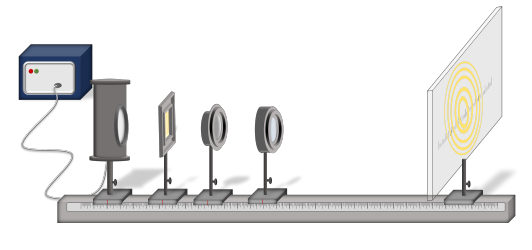
\includegraphics[width=0.8\textwidth, height = 4cm, scale=3.0]{Bilder/Titelbild O3.png}   %Bild ändern
\end{center}      
    \vfill
\end{titlepage}
\setcounter{page}{2}



\pagestyle{fancy}
\markboth{INHALTSVERZEICHNIS}{}
\tableofcontents
\newpage

\pagestyle{fancy}
\justifying
\section{Einleitung}


\newpage
\section{Theoretische Grundlagen}

%\begin{wrapfigure}{r}{0.4\textwidth} % r=rechts, l=links, 0.4=Breite 
%        \centering
%        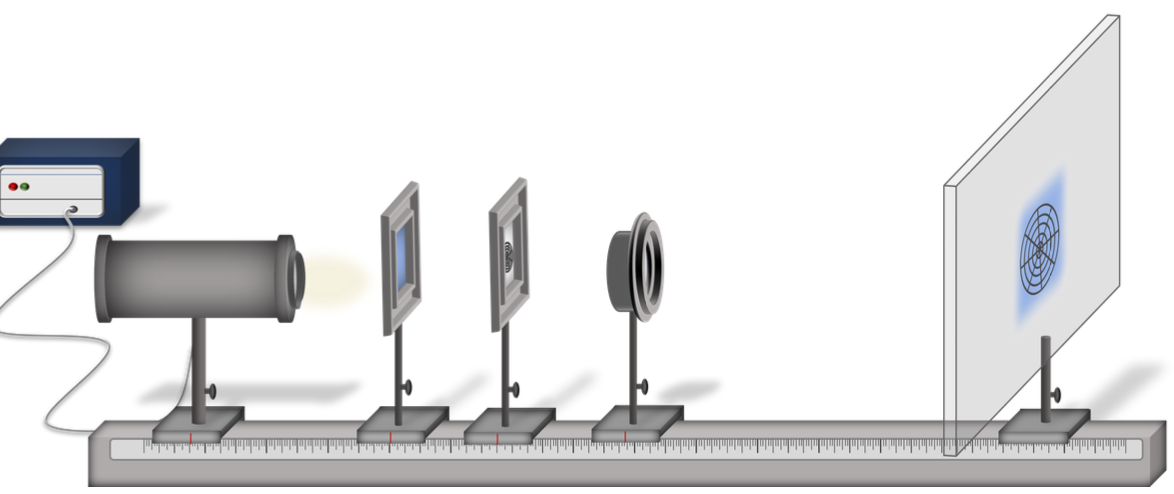
\includegraphics[width=0.9\linewidth]{Bilder/Titelbild.png}
%        \caption{Veranschaulichung der LSA}
%       \label{fig:SpASkizze}
%\end{wrapfigure}

\subsection{Lichtbrechung}
Das für uns sichtbare Licht besteht aus vielen Wellenlängen an 
Elektromagnetischen Wellen. Damit diese verschiedenen Wellenlängen 
einzeln betrachtet werden können, kann man das sichtbare Licht 
mithilfe eines optischen Prismas brechen. Dieser Vorgang kann in 
Abbildung 1 beobachtet werden. Die verschiedenen Brechungswinkel 
hängen mit den unterschiedlich starken brechungen der 
unterschiedlichen Elektromagnetischen Wellen zusammen. 
Diese Brechung ist als Brechungsindex bekannt. Der Zusammenhang 
zwischen Brechungsindex und der Wellenlängen der 
Elektromagnetischen Welle wird an einem späteren Zeitpunkt noch 
genauer betrachtet.
\begin{figure}[!htb]
\centering
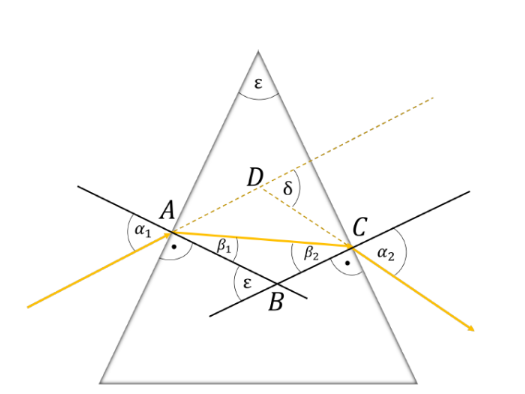
\includegraphics{Bilder/Strahlengang O2.png}
\caption{Abbildug 1: Der Strahlengang eines gebrochenen Lichtstrahles innerhalb eines Prisma mit den wichtige Winkeln}
\end{figure}

Um den Brechungsindex für einzenlne Wellenlängen bestimmen zu 
können, betrachtet man zunächst den Ablenkungswinkel $\delta$. 
Dieser wird minimal für $\alpha_1 = \alpha_2$ und $\beta_1 = 
\beta_2$ womit für beide Winkel
\begin{equation}
    \beta_1 = \frac{\varepsilon}{2}
    \label{eq:1}
\end{equation}

und

\begin{equation}
    \alpha_1 = \frac{\delta_{\text{min}} + \varepsilon}{2}
    \label{eq:2}
\end{equation}
gilt. Wenn diese gleichungen nun mit dem snelliusschen Brechungsgesetz kombiiert werde

\begin{equation}
    n_1 \cdot \sin(\alpha_1) = n_2 \cdot \sin(\beta_1)
    \label{eq:3}
\end{equation}

mit $n_1 = n_{\text{Luft}} \stackrel{!}{=} 1$ und den Winkeln aus Gleichung (\ref{eq:1}) und (\ref{eq:2}) folgt für den Brechungsindex $n$ des Prismas

\begin{equation}
    n = n_2 = \frac{\sin\left(\frac{\delta_{\text{min}} + \varepsilon}{2}\right)}{\sin\left(\frac{\varepsilon}{2}\right)} .
    \label{eq:4}
\end{equation}


\subsection{Dispersion}
Dispersion beschreibt in dem betrachteten Fall den Zusammenhang 
zwischen der Wellenlänge der betrachteten Elektromagnetischen 
Wellen und des Brechungsindex. Diese Abhängigkeit lässt sich am 
Thomson-Atommodel erkären. Dieses Atommodel beschreibt ein Atom 
als homogen positiv geladene Kugel in der die elektronen frei 
beweglich sind. In diesem Modell können Elektronen durch 
Elektromagnetische Wellen zu Schwingungen angeregt werden. 
Diese Schwingung lässt sich durch die folgenden Differential 
Gleichung beschrieben werden. 
\begin{center}
    $m_0r*\ddot{r} + m\gamma*\dot{r} + m_0*\omega_0^2*r=-e*E$
\end{center}
wobei $\omega_0$ die Eigenfrequenz der Elektronen beschreibt, 
$m_0*\gamma*\dot{r}$ ist die Darstellung des Dämpungsterm, e die 
Elementarladung und E die Elektrische Feldstärke des anregenden 
Photons.\\
Bei der Dispersion können drei Fälle auftreten. Der erste Fall 
ist für $\omega<<\omega_0$, bei diesem Fall kann man die Dämpfung 
vernachlässigen, und es kommt zu normaler Dispersion. Bei 
$\omega\approx \omega_0$ kommt es zu anomaler Dispersion. Der 
letzte Fall ist bei $\omega_0 << \omega$, dieses Ereigniss ist 
als Resonanzkatastrophe bekannt und tritt zum Beispiel auf, wenn 
eine Armee im Gleichschritt über eine große Brücke marschiert. 
Bei diesem Experiment sind aber nur die normale und anomale 
Dispersion wichtig. Bei normaler Dispersion nimmt der 
Brechungsindex mit steigender Frequenz/sinkender Wellenlänge zu, 
während bei der anomalen Dispersion genau das Gegenteil geschieht 
dort nimmt der Brechungsindex bei steigender Wellenlänge zu.

\newpage
\section{Versuchsbeschreibung}
\subsection{Versuchsaufbau}
%\begin{wrapfigure}{r}{0.4\textwidth} % r=rechts, l=links, 0.4=Breite 
%        \centering
%        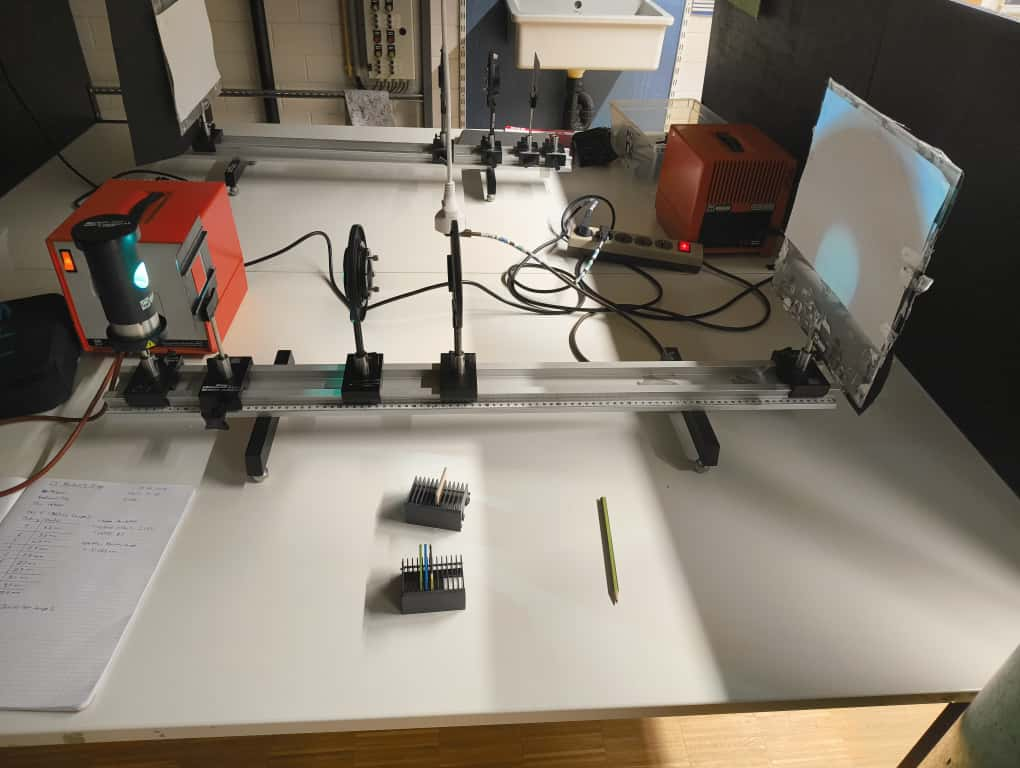
\includegraphics[width=0.9\linewidth]{Bilder/Versuchsaufbau O3.jpeg}
%        \caption{Versuchsaufbau}
%       \label{fig:SpASkizze}
%\end{wrapfigure}


\subsection{Versuchsdurchführung}

\newpage
\section{Auswertung}
\newpage
\section{zusammenfassung}
\newpage
\section{Anhang}
\newpage
\section{Literaturverzeichnis}



\end{document}
